\section{Atom wodoru}
\subsection{Wstęp}
Przypomnijmy sobie czym jest atom wodoru. Mamy jeden atom i mamy jeden wektor, dwa ciała które ze sobą współdziałają, jakieś cząstki A oraz B. Pytanie czy możemy jakoś zredukować to zagadnienie do jedno-cząstkowego zagadnienia? Odpowiedź brzmi że faktycznie możemy. Najpierw możemy wypisać że potencjał współdziałania między tymi cząstkami rozpisujemy jako 
$$
V(\vec{r}_A, \vec{r}_B) = V(\vec{r})
$$
gdzie $\vec{r} = \vec{r}_A - \vec{r}_B$. Hamiltonian będzie wtedy wyglądał następująco
\begin{equation*}
	H =  \frac{p_{A}^{2}}{2 m_{A}}+\frac{p_{B}^{2}}{2 m_{B}} + V(\vec{r} _A- \vec{r}_B)
\end{equation*}
Równanie Schrödingera dla tego układu natomiast będzie wyglądać tak
\begin{equation*}
	i \hbar \frac{\partial}{\partial t} \psi \left(\vec{r}_{A}, \vec{r}_{B}, t\right) = \left[-\frac{\hbar^{2}}{2 m_{A}} \vec{\nabla}_{A}^{2}+V(\vec{\nu})\right] \psi \left(\vec{r}_{A}, \vec{r}_{B}, t\right)
\end{equation*}
Jak teraz to uprościć? Możemy wprowadzić promień położenia	
\begin{equation*}
	\vec{R}=\frac{m_{A} \vec{r}_{A}+m_{B} \vec{r}_{B}}{m_{A}+m_{B}}, \quad m = m_A + m_B
\end{equation*}
A również wprowadzamy tak zwaną masę zredukowaną
\begin{equation*}
	\mu = \frac{m_A m_B}{m_A + m_B}
\end{equation*}
W takim razie równianie schrodingera będze wyglądało następująco
\begin{align*}
	&\left.
	\begin{aligned}
		i \hbar\dot{\psi}(\bar{R}, \bar{r}, t)  =  \left[-\frac{\hbar^{2}}{2 M} \nabla_{R}^{2}-\frac{\hbar^{2}}{2 \mu} \nabla_{2}^{2}+V(\vec{r})\right]  \psi(\bar{R}, \bar{r}, t) \\
		\psi(\vec{R}, \vec{r}, t)=\phi(\vec{R}) \psi(\vec{r}) \exp \left(\frac{-[E_m + E]t}{\hbar}\right)
	\end{aligned}
	\right\}
	\xRightarrow[\text{zmiennych}]{\text{Metoda rozdzielnych}}
\end{align*}
\begin{align*}
	\xRightarrow[\text{zmiennych}]{\text{Metoda rozdzielnych}}
	&\left\{
	\begin{aligned}
		&\frac{-\hbar^{2}}{2 m} \nabla_{R}^{2} \phi(R)=E_{CM} \phi(R)\\
		&\left[\frac{-\hbar^{2}}{2 M} \nabla_{2}^{2}+\nabla(\vec{r})\right] \psi(\vec{r})=E \psi(\vec{r})
	\end{aligned}
	\right.
\end{align*}
Są dwie klasy zagadnień dla których to równanie ma ciekawe rozwiązanie.
W pierwszym przypadku weźmy oscylator harmoniczny
\begin{equation*}
	V(\vec{r})=\frac{1}{2} k_{1} x^{2}+\frac{1}{2} k_{2} y^{2}+\frac{1}{2} k_{3} z^{2}, \quad \vec{r} = (x, y, z)
\end{equation*}
W przypadku gdy mamy potencjał centralny to on będzie wyglądał następująco
\begin{equation*}
	V(\vec{R}) = V(\overline{|r|}) = V(r)
\end{equation*}
Będziemy pisać $r$ bez strzałki i to po prostu oznacza długość wektora r. To jest tak zwany potencjał centralny i w tym przypadku wygodnie jest przejść do współrzędnych sferycznych. Wtedy Hamiltonian będzie wyglądał tak
\begin{equation*}
	\begin{split}
			H &=\frac{-\hbar^{2}}{2 \mu} \nabla^{2}+V(r) \\
			&= \frac{-\hbar^{2}}{2 \mu} \left[ \frac{1}{r^{2}} \frac{\partial}{\partial r} \left( r^{2} \frac{\partial}{\partial r} \right) + \frac{1}{r^{2} \sin \theta} \frac{\partial}{\partial \theta} \left( \sin \theta \frac{\partial}{\partial \theta} \right) + \frac{1}{r^{2} \sin^{2} \theta} \frac{\partial^{2}}{\partial \phi^{2}} \right] +V(r) \\
			&= -\frac{\hbar^2}{2\mu} \left[ \frac{1}{r^2} \frac{\partial}{\partial r} \left( r^2 \frac{\partial}{\partial r} \right) - \frac{1}{\hbar^2 r^2} \hat{L}^2 \right] + V(r)
	\end{split}
\end{equation*}
Wstawiając to do RS dostajemy
\begin{equation*}
	\left[ -\frac{\hbar^2}{2\mu} \left( \frac{1}{r^2} \frac{\partial}{\partial r} \left( r^2 \frac{\partial}{\partial r} \right) - \frac{1}{\hbar^2 r^2} \hat{L}^2 \right) + V(r) \right] \psi(\vec{r}) = E \psi(\vec{r})
\end{equation*}
Dalej pamiętamy, że w przypadku gdy mamy jakąś funkcję współrzędnych to ta funkcja komutuje z operatorem $\hat{L}_x$ albo $\hat{L}_x$ albo $\hat{L}_x$ i tak samo z operatorem $\hat{L}^2$. 
\begin{equation*}
	\begin{split}
		[\hat{L}_x, \hat{f}(r)] = 0 \\
		[\hat{L}_y, \hat{f}(r)] = 0 \\
		[\hat{L}_z, \hat{f}(r)] = 0 \\
		[\hat{L}^2, \hat{f}(r)] = 0 
	\end{split}
\end{equation*}
\text{Pytanie z sali:} jak mamy rozumieć ten zapis? \textbf{Odp.} to jest operator który jest zależny od $r$
Wprowadzamy teraz założenie jak będzie wyglądała nasza funkcja. Mówimy że rozwiązanie poprzedniego równania będzie miało kształt
\begin{equation*}
	\psi_{Elm} = R_{Elm}(r) \psi_{lm}(\Theta, \Phi)
\end{equation*}
Wrzucamy to wszystko do równania Schrödingera i dostajemy
\begin{align*}
	&\left\{
	\begin{aligned}
		&L^2 \psi_{lm}(\Theta, \Phi) =  l(l+1) \hbar^2 \psi_{lm}(\Theta, \Phi)\\
		&\left[-\frac{\hbar^2}{2\mu} \left(\frac{\text{d}^2}{\text{d}r^2} + \frac2r \frac{\text{d}}{\text{d}r} \right) + \frac{l(l+1)\hbar^2}{2 \mu r^2} + V(r)\right] R_{Elm} = E R_{lm}
	\end{aligned}
	\right.
\end{align*}
Powiedzmy teraz że będziemy pisać $U_{EL}(r) = r \cdot R_{EL}(r)$ i wtedy RS będzie pisane tak
\begin{equation*}
	\begin{gathered}
		-\frac{\hbar^2}{2\mu}\frac{d^2 U_{EL}(r)}{dr^2}+V_{eff}(r)U_{EL}(r)=EU_{EL}(r) \\
		V_{eff} = V(r)+\frac{l(l+1)\hbar^2}{2\mu r^2}
	\end{gathered}
\end{equation*}
\subsection{Wodór}
Dla wodoru potencjał będzie wyglądał następująco
\begin{equation*}
	\begin{gathered}
		V(r)=-\frac{z e^{2}}{\left(4 \pi \varepsilon_{0}\right)^2}\\
		V_{eff}(r) = -\frac{z e^2}{4 \pi \varepsilon_0 r} + \frac{l(l+1)\hbar^2}{2\mu r^2}
	\end{gathered}
\end{equation*}
Gdzie "$z$" to jest ładunek jądrowy (1 dla wodoru, 2 dla pierwszego jony Helu i tak dalej). Wrzucamy to wszystko znowu do równania Schrödingera ale przed tym zdefiniujemy sobie zmienne do ułatwienia zapisu
\begin{equation*}
	\begin{gathered}
		\rho=\left(\frac{-8\mu E}{\hbar^2}\right)^{1/2}r\\
		\lambda = \frac{Z e^2}{(4 \pi \epsilon_0) \hbar} \left(\frac{-\mu}{2E}\right)^{1/2}
	\end{gathered}
\end{equation*}
Wtedy RS się przekształci w 
\begin{equation*}
	\left[\frac{d^{2}}{d \rho^{2}}-\frac{l(l+1)}{\rho^{2}}+\frac{\lambda}{\rho}-\frac{1}{4}\right]U_{El(\rho)}=0
\end{equation*}
Chcemy zrozumieć jak będą wyglądały nasze rozwiązania. Podejście będzie analogiczne jak kiedy rozwiązywaliśmy dla oscylatora harmonicznego. Najpierw chcemy zrobić jak będzie wyglądało rozwiązane asymptotyczne gdy $\rho \to \infty$, wtedy 
\begin{equation*}
	\left[\frac{\text{d}^{2}}{\text{d} \rho^{2}}-\frac{1}{4}\right]U_{El(\rho)}=0
\end{equation*}
Równanie to daje nam możliwość zapisania jak będzie wyglądać $U_{El}$ gdy $\rho$ dąży do nieskończoności
\begin{equation*}
	U_{El(\rho)} \xrightarrow[\rho \to \infty]{} \exp(\frac{-\rho}{2})
\end{equation*}
Mając to możemy założyć że
\begin{equation*}
	U_{El(\rho)} = \exp(\frac{-\rho}{2}) \cdot f(\rho)
\end{equation*}
No i teraz możemy to wrzucić do RS i będziemy mieli
$$  \left[\frac{d^{2}}{d \rho}-\frac{d}{d \rho}-\frac{l(l+1)}{\rho^{2}}+\frac{\lambda}{\rho}\right] f(\rho)=0  $$
Dalej robimy że $f(\rho) = \rho^{l+1}g(\rho)$. Teraz będziemy chcieli zrozumieć jakie będą wartości własne operatora Hamiltona, i do tego nie potrzebujemy całkowitego rozwiązania tylko takie rozwiązanie które określi warunki na znaczenie tych wartości własnych, i dlatego znowu rozkładamy funkcje $g(\rho)$ w szereg.
\begin{equation*}
	g(\rho)=\sum_{k=0}^{\infty} c_{k} \rho^{k}, \quad c_0 \neq 0
\end{equation*}
Wrzucamy najpierw podstawienie $f(\rho) = \rho^{l+1}g(\rho)$ i mamy
\begin{equation*}
	\left[\rho\frac{\text{d}^{2}}{\text{d} \rho}+(2l + 2 - \rho)\frac{\text{d}}{\text{d} \rho} + (\lambda - l - 1)\right] g(\rho)=0
\end{equation*}
Jeżeli teraz dodamy założenie o postaci $g(\rho)$ dostaniemy
\begin{equation*}
	\sum_{k=0}^{\infty}\left[ \left( k(k+1) + (2l+2)(k+1) \right)C_{k+1} + (\lambda - l - 1 -k)C_k \right]\rho^k=0
\end{equation*}
Skoro suma jest zerem to każdy składnik jest zerem więc możemy z tego wyznaczyć
\begin{equation*}
	C_{k+1} = \frac{-(\lambda - l - 1 -k)}{(k+1)(2l+2+k)} C_k
\end{equation*}
Mamy też $\frac{C_{k+1}}{C_k} \xrightarrow{k \to \infty} \frac{1}{k}$ przez co mamy niezbieżność, ten sam problem co mieliśmy w przypadku oscylatora harmonicznego. Teraz musimy odciąć w takim razie ten nasz szereg w jakimś punkcie, to znaczy musi istnieć jakieś $\lambda$ dla którego ten współczynnik będzie po prostu zero dla jakiegoś $k$. Mówimy że niech istnieje taki $r_n:C_{r_n}= 0$. W takim razie teraz mamy
\begin{equation*}
	\begin{gathered}
		r_n+ l +1 - \lambda = 0 \\
		\lambda = r_n + l +1
		\text{Niech} n = \lambda = r_n + l +1
	\end{gathered}
\end{equation*}
Powyżej $n$ nazywamy główną liczbą kwantową. Tutaj możemy zobaczyć że mamy kilka warunków, że $l \in \mathcal{N}$, z tego wynika że $0 \leq l \leq n - 1$. Teraz wstawiamy to co mieliśmy 
\begin{equation*}
	\begin{split}
		&\lambda = n = \frac{Z e^2}{(4 \pi \epsilon_0) \hbar} \left(\frac{-\mu}{2E}\right)^{1/2} \\
		&\Rightarrow E_n = \frac{\mu}{2\hbar^2} \left( \frac{ze^2}{4 \pi \epsilon_0} \right)^2 \frac{1}{\hbar^2} \\
		&\Rightarrow \frac{-1}{2}\mu c^2 \frac{(z\alpha)^2}{n^2}, \quad n = 1, 2, 3, \dotsc
	\end{split}
\end{equation*}
Gdzie $\alpha$ to jest stała, tak zwana stała struktury. Widzimy tutaj że Energia zależy $n$ i nie jest zależna $l$. Wcześniej pisaliśmy energię w równaniu z $l$, jednak teraz widzimy że wartości własne nie zależą od $l$.

Możemy zapisać że $ l\in(0,1,\ldots,n-1) $, $ m\in(-l,\ldots,l) $ i $n\in(1, 2, \dotsc)$. Biorąc to wszystko pod uwagę możemy narysować poziomy energii
\begin{figure}[H]
	\centering
	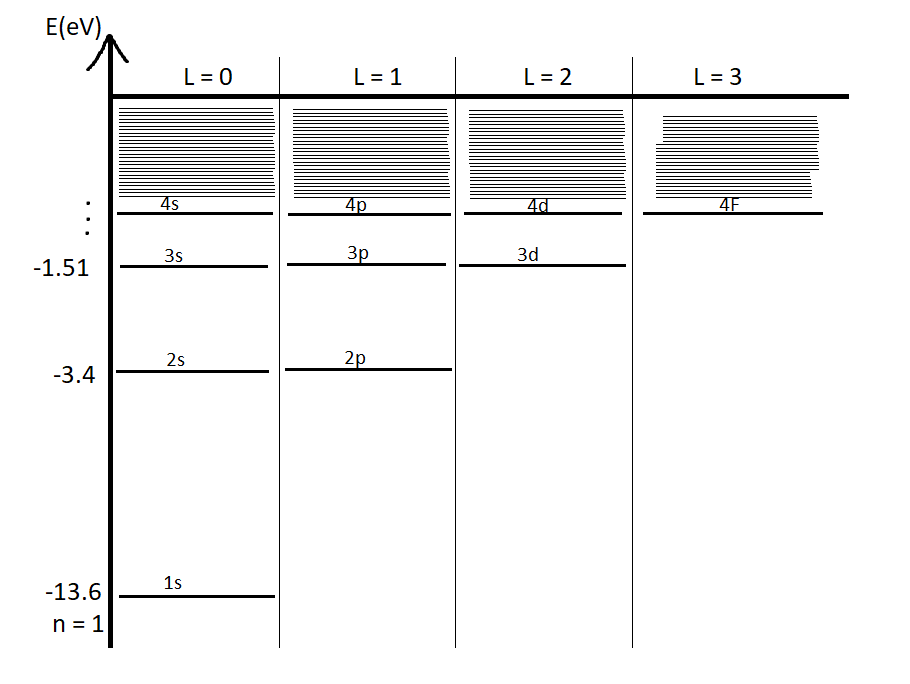
\includegraphics[width=0.7\textwidth]{poziomyenergii}
	\caption{Poziomy energii.}
	\label{fig:poziomyenergii}
\end{figure}
\subsection{Stany własne}
Wracamy teraz dla równania po podstawieniu funkcji $g(\rho)$
\begin{equation*}
	\left[\rho\frac{\text{d}^{2}}{\text{d} \rho}+(2l + 2 - \rho)\frac{\text{d}}{\text{d} \rho} + (\lambda - l - 1)\right] g(\rho)\neq0
\end{equation*}
Chcielibyśmy wprowadzić nowe zmienne żeby to przekształcić do równania
\begin{equation*}
	z \frac{d w}{d z^{2}}+(c-z) \frac{d w}{d z}-a w=0 
\end{equation*}
Jest to tak zwane równanie Kummer'a-Laplace'a. Musimy wprowadzić w takim razie
\begin{equation*}
	\begin{gathered}
		z \equiv \rho \\
		w \equiv g \\
		a \equiv l + 1 - \lambda \\
		c \equiv 2l + 2
	\end{gathered}
\end{equation*}
To równanie jest nam potrzebne ponieważ znamy rozwiązanie tego równania i są to funkcje hiper geometryczne. Są one definiowane następująco
\begin{equation*}
	\prescript{}{1}{F}_{1}(a, c, z)=1+\frac{a z}{c\cdot1!}+\frac{a(a+1) z^{2}}{c(c+1) 2!}+\ldots=\sum_{k=0}^{\infty} \frac{(a)_{k} z^{k}}{(c)_{k} k!}
\end{equation*}
Gdzie $(\alpha)_k = \alpha (\alpha+1)\dotsc(\alpha+k-1)$, $(\alpha)_0=1$. Asymptotyczne zachowanie tej funkcji dla $z \to \infty$ jest następujący
\begin{equation*}
	\prescript{}{1}{F}_{1}(a, c, z) \xrightarrow[z \to \infty]{} \frac{\Gamma(c)}{\Gamma(a)}e^z z^{a-c}
\end{equation*}
Teraz kiedy podstawiamy wszystko mamy
\begin{equation*}
	\prescript{}{1}{F}_{1}(l + 1 - n, 2l+2, \rho) \rightarrow \rho^{-l-1-\lambda} e^{\rho}
\end{equation*}
Jaki mamy tu problem? Ta funkcja jest rozbieżna. Musimy z tym szeregiem popracować i znowu gdzieś go odciąć. Mianowicie musimy znowu wyzerować licznik więc znowu $l + 1 - \lambda = -r_n$ i z tego
\begin{equation*}
	\prescript{}{1}{F}_{1}(l + 1 - n, 2l+2, \rho) = \sum_{n=0}^{n - l -1} \frac{(k+l - n)(k -1+l-n)\dots(l+1-n)}{(k+2l+1)(k-1+2l - n)\dots(1 + 2l - 1)} \frac{\rho^k}{k!}
\end{equation*}
I niby mamy rozwiązanie ale tyle nam nie wystarczy, chcemy wyprowadzić jeszcze to przez wielomiany Laguerre'a które mają następującą definicje
\begin{equation*}
	\begin{split}
		L_q^p(\rho)&= \frac{d^p}{d \rho^p}L_q(\rho) \\
		L_q(\rho) &= e^{\rho} \frac{d^q}{d \rho^q}\left(\rho^q e^{-\rho}\right)
	\end{split}
\end{equation*}
To są wielomiany Laguerre'a i możemy rozpisać związek między funkcjami hiper geometrycznymi a wielomianem Laguerre'a.
\begin{equation*}
	L_{n+l}^{2l+1}(\rho) = -\frac{[(n+l)!]^2}{(n-l-1)!(2l+1)!} \prescript{}{1}{F}_{1}(l + 1 - n, 2l+2, \rho) 
\end{equation*}
Zapiszmy teraz już końcowe rozwiązanie w postaci funkcji radialnej $R$.
\begin{equation*}
	\begin{gathered}
		R_{n l}(\rho)=N \cdot e^{\frac{-\rho}{2}} \rho^{l} L_{n+l}^{2 k+1}(\rho), \quad \text{gdzie} \\
		\rho=\left(\frac{-8\mu E}{\hbar^2}\right)^{1/2}r \\
		N = \left( \left( \frac{2Z}{n a_{\mu}} \right) \frac{(n - l - 1)!}{2n[(n+1)!]^3} \right)^{\frac{1}{2}} \\
		a_{\mu} = \left(\frac{4 \pi \epsilon_0 \hbar^2}{\mu e^2}\right)
	\end{gathered}
\end{equation*}
Teraz wypiszemy pierwsze trzy funkcje i naszkicujemy.
\begin{equation*}
	\begin{split}
		R_{1,0}(r) &=  2 \left(\frac{Z}{a_{\mu}}\right)^{\frac32} \exp(-\frac{zr}{a_{\mu}}) \\
		R_{2,0}(r) &=  2 \left(\frac{Z}{2a_{\mu}}\right)^{\frac32}\left(1 - \frac{zr}{2a_{\mu}}\right) \exp(-\frac{zr}{a_{\mu}}) \\
		R_{2,0}(r) &=  \frac{1}{\sqrt(3)} \left(\frac{Z}{2a_{\mu}}\right)^{\frac32} \left(\frac{zr}{a_{\mu}}\right) \exp(-\frac{zr}{a_{\mu}})
	\end{split}
\end{equation*}
Od razu możemy pomyśleć o tym jakie będzie średnie położenie cząstki
\begin{figure}[htb]
	\centering
	\begin{minipage}[t]{0.47\textwidth}
		\centering
		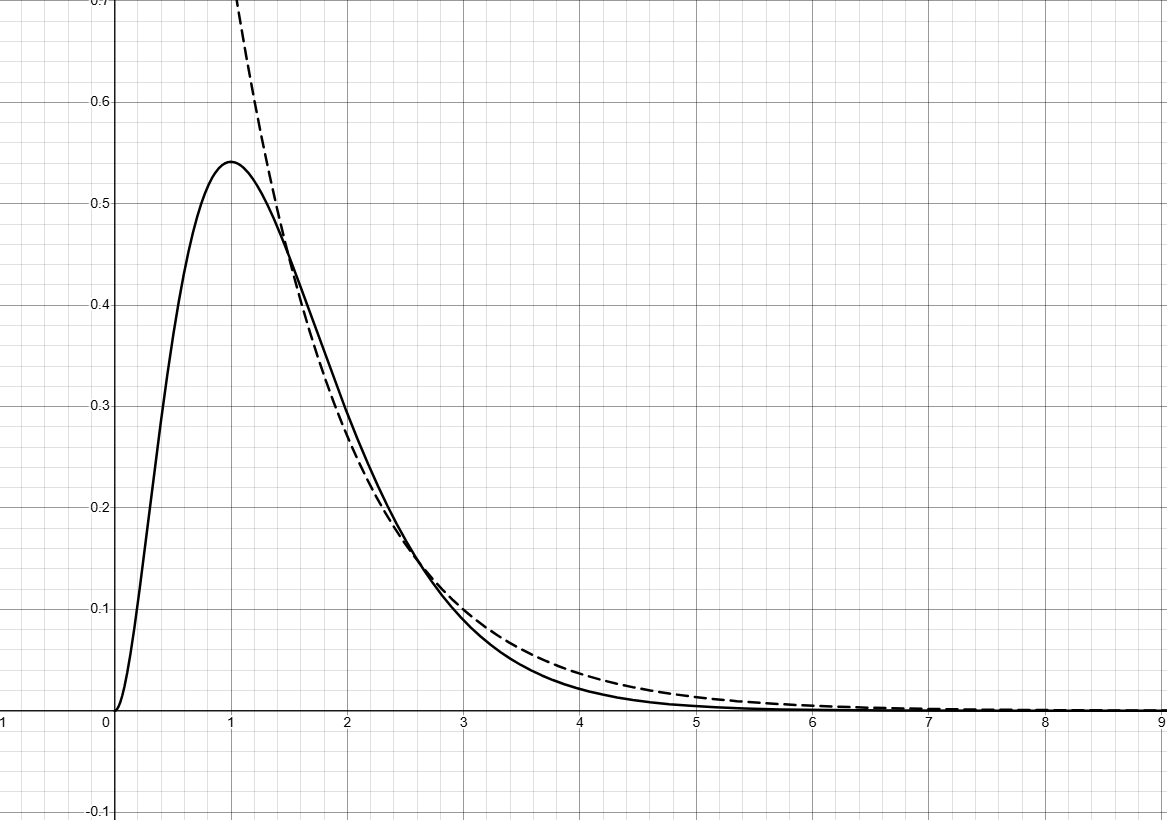
\includegraphics[width=\linewidth]{R10}
		\caption{Wykres $R_{1, 0}$}
		\label{fig:R10}
	\end{minipage}
	\hspace{0.04\textwidth}
	\begin{minipage}[t]{0.47\textwidth}
		\centering
		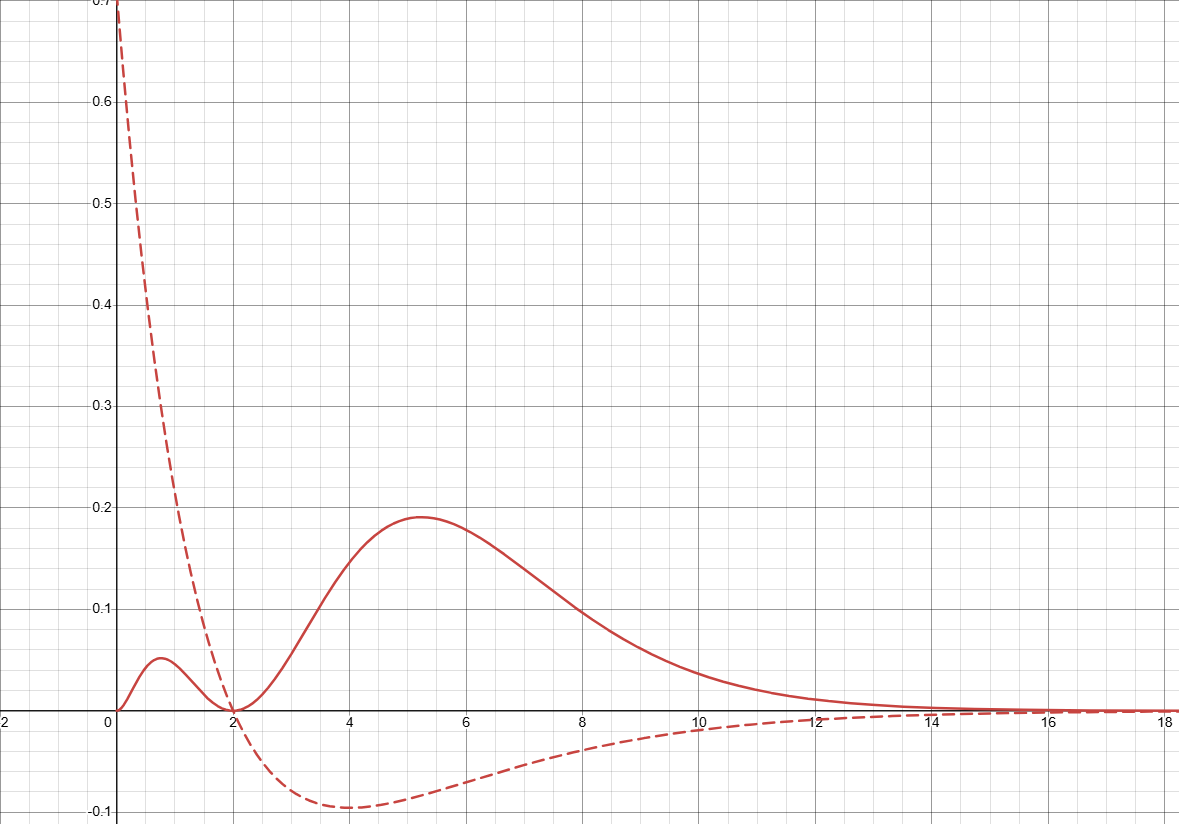
\includegraphics[width=\linewidth]{R20}
		\caption{Wykres $R_{2, 0}$}
		\label{fig:R20}
	\end{minipage}
\end{figure}
\begin{figure}[htb]
	\centering
	\begin{minipage}[t]{0.47\textwidth}
		\centering
		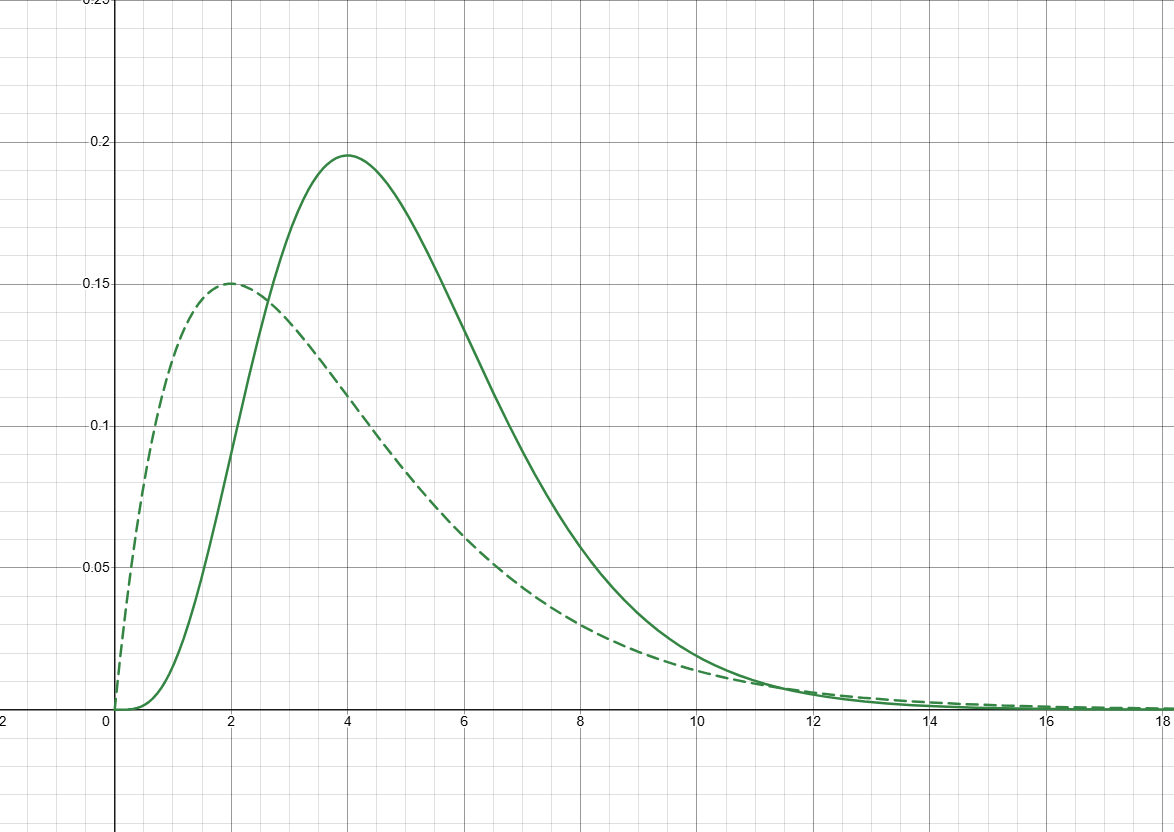
\includegraphics[width=\linewidth]{R21}
		\caption{Wykres $R_{2, 1}$}
		\label{fig:R21}
	\end{minipage}
	\hspace{0.04\textwidth}
	\begin{minipage}[t]{0.47\textwidth}
		\centering
		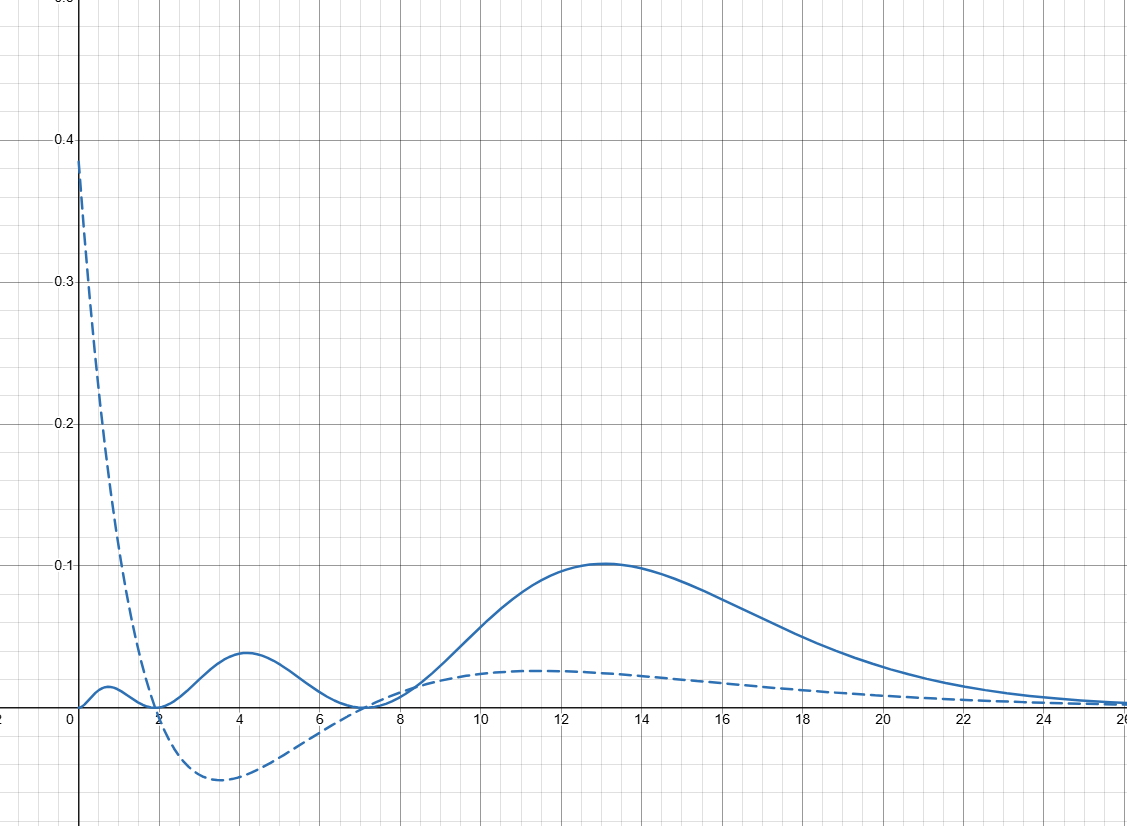
\includegraphics[width=\linewidth]{R30}
		\caption{Wykres $R_{3, 0}$}
		\label{fig:R30}
	\end{minipage}
\end{figure}

Te wykresy pokazują że średnie położenie cząstki musi poruszać się "w prawo" gdy zwiększamy $r$.
